\chapter{Korrektheit}

In diesem Kapitel stellen wir, die von uns definierten Korrektheitskriterien, mit dessen Hilfe die Korrektheit von unseren Unparser bewerten werden kann. Es gibt auch eine Auswertung, wo die Korrektheitskriterien auf die Implementierung unseren Algorithmen angewandt werden. \\

Wir stellen unsere Definitionen der Korrektheitskriterien vor. Es werden jeweils Korrektheitskriterien für textbasierte Diffs und C-Präprozessor-Annotierten Code definiert. Danach werden die Korrktheitskriterien näher beschrieben. Die Zusammenhänge zwischen den Korrektheitskriterien werden gezeigt. Bei der Auswertung wird der Aufbau und Ergebnisse beschrieben. Basierend auf dem wird die Forschungsfrage und Ergebnisse diskutiert.\\

In Kapitel 5.1 werden die Korrektheitskriterien definiert, näher beschrieben und die Zusammenhänge zwischen den dargestellt. Die Auswertung mit dem Aufbau des Experiments, den Ergebnissen und der Diskussion sind in dem Kapitel 5.2 zu finden.




\section{Korrektheitskriterium}

%In diesem Kapitel stellen wir die Metrik vor, an der wir die Korrektheit unserer Lösung betrachten wollen. Dieser Kapitel beschäftigt sich nur mit Arten der Korrektheit und wie diese als Konzept für textbasierte Diffs und mit C-Präprozessor-Annotierten Code funktionieren soll. Die drei Arten der Korrektheit für textbasierte Diffs und mit C-Präprozessor-Annotierten Code, sind syntaktische Korrektheit, syntaktische Korrektheit ohne Whitespace und semantische Korrektheit, werden in diesem Kapitel erläutert.\\

%Nachdem wir eine algorithmische Lösung für das Problem ausgearbeitet haben, müssen wir entscheiden, ob unsere Lösung korrekt ist. Um die Kriterien, an den die Korrektheit festgelegt wird, wird es in folgenden gehen. Wir stellen Ihnen unsere Metrik für die Korrektheit des Unparsens. Wir haben uns für drei mögliche Arten der Korrektheit entschieden, an denen wir die Korrektheit entscheiden. Diese Arten sind syntaktische Gleichheit, syntaktische Gleichheit ohne Whitespace und semantische Gleichheit. Wenn die ausgangs Eingabe und das Ergebnis der ausgangs Eingabe nach Parsen und Unparsen eine dieser Gleichheiten erfühlen gilt das Unparsen für diesen Fall als Korrekt. In der Tabelle 4.1 ist kurz zusammengefasst wie jeweils die Art der Korrektheit bezogen auf C-Präprozessor-Annotierter Code oder textbasierte Diffs zu verstehen sind.


Nachdem wir unseren Algorithmus in DiffDetective implementiert haben, müssen wir noch feststellen wie Korrekt unsere Implementierung ist. Dazu müssen wir zuerst definieren, wie wir die Korrektheit unsrer Implementierung verstehen. Deshalb haben wir Korrektheitskriterien für textbasierte Diffs und C-Präprozessor-Annotierten Code aufgestellt, um die es in diesem Abschnitt geht.\\

Die Bewertung der Korrektheit unseren Unparser, geht wie folgt. Es wird ein C-Präprozessor-Annotierter Code oder textbasierter Diff genommen. Dieser C-Präprozessor-Annotierter Code oder textbasierter Diff wird ungeparst und wir erhalten ein Variation-Tree oder ein Variation-Diff. Der Variation-Tree oder Variation-Diff wird im Nächsten Schritt ungeparst und wir erhalten wieder ein C-Präprozessor-Annotierten Code oder textbasierten Diff. Zum Schluss werden der ausgangs C-Präprozessor-Annotierter Code mit dem ungeparsten C-Präprozessor-Annotierter Code oder der ausgangs, textbasierter Diff mit dem ungeparsten, textbasierten Diff anhand der von uns definierte Korrektheitskriterien verglichen und entschieden, ob korrekt ungepasrt wurde oder nicht.\\

Die von uns definierten Korrektheitskriterien sind syntaktische Gleichheit, syntaktische Glichheit ohne Whitespace und semantische Gleichheit. Die formale Definition der Korrektheitskriterien ist in der Tabelle 5.1 zu sehen. Diese Tabelle zeigt in der ganz linken Spalte, die Bezeichnungen der Korrektheitskriterien und die ganz obere Zeile zeigt, worauf diese Korrektheitskriterien angewandt werden können. Die anderen Zellen zeigen wie das Korrektheitskriterium auf C-Präprozessor-Annotierten Code bzw. textbasierten Diff angewandt werden kann. In der Zelle der zweiten Zeile und zweiten Spalte werden die Funktionen $parse_t$ und $unparse_t$ für Variation-Trees und C-Präprozessor-Annotierten Code definiert. Außerdem wird definiert das die Verkettung der Funktionen $parse_t$ und $unparse_t$ gleich der Identitätsfunktion ist. Das stellt die Definition der syntaktischen Gleichheit für C-Präprozessor-Annotierten Code dar. Der Inhalte der Zelle der zweiten Zeile und dritten Spalte ist analog zu Inhalt vorher beschriebenen Zelle, aber in dieser Zelle werden die Funktionen für Variation-Diffs und textbasierte Diffs definiert und diese Zelle enthält die Definition der syntaktischen Gleichheit für textbasierte Diffs. In der Zelle der dritten Zeile und zweiten Spalte befindet sich die Definition der syntaktischen Gleichheit für C-Präprozessor-Annotierten Code. Dort werden die Funktionen definiert und es kommt eine neue Funktion hinzu. Das ist $deleteWhitespace_t$, welche auf einer bestimmten Art und Weise bestimmte Whitespace-Zeichen entfernt, so das C-Präprozessor-Annotierten Code erhalten bleibt und nicht zu einem willkürlichen Text wird. Hier wird definiert, dass die Verkettung von $deleteWhitespace_t$, $unparse_t$ und $parse_t$ gleich der Verkettung von $deleteWhitespace_t$ und $id$ ist. Der Inhalt der Zelle von dritter Zeile und dritter Spalte ist analog zu der Zelle aus der dritten Zeile und zeiten Spalte. In dieser Zelle wird die syntaktische Gleichheit für textbasierte Diffs definiert. Der Unterschied zu dem vorherigen ist das hier die Funktionen $deleteWhitespace_d$, $unparse_d$ und $parse_d$ verwendet werden, welche mit textbasierten Diffs und Variation-Diffs arbeiten. Es wird trotzdem definiert, dass die Verkettung von $deleteWhitespace_d$, $unparse_d$ und $parse_d$ gleich der Verkettung von $deleteWhitespace_d$ und $id$ ist. Der Inhalt der Zelle in der Zelle der vierten Zeile und dritten Spalte sollte die Definition der semantischen Gleichheit für C-Präprozessor-Annotierten Code sein. Die  Erarbeitung so einer Definition geht über den Rand unserer Möglichkeiten hinaus, deshalb haben wir das nicht gemacht. In der Zelle der vierten Zeile und dritten Spalte der Tabelle 5.1, befindet sich die Definition der semantischen Gleichheit für textbasierte Diffs, welche wie folgt aussieht. Zuerst werden die benötigten Mengen definiert, danach die benötigten Funktionen. Zu den benötigten Funktionen gehören $deleteWhitespace_t$, $unparse_d$, $parse_d$ und $textProject$. Alle Funktionen außer $textProject$ sind gleich zu den Funktionen aus anderen Definitionen. Die Funktion $textProtect$ erhält, einen textbasierten Diff und eine Zeit als Eingabe und Projeziert und wir erhalten als Ausgabe ein C-Präprozessor-Annotierter Code, welche die Projektion des textbasierten Diff auf die Zeit darstellt, so wie die Projektion bei Variation-Diff nur für textbasierte Diff. Zum Schluss steht wie die semantische Gleichheit für textbasierte Diff zu verstehen ist. Diese Definition ist wie folgt zu verstehen, wenn die Ausgaben der Funktionen $textProject$ für alle Zeiten $t$ und alle textbasierte Diff $d$ gleich sind, nachdem auf $d$ die Verkettung von $unparse_d$ und $parse_d$ bzw. $id$ angewandt wurde oder wenn zusätzlich dazu  $textProject$ mit  $deleteWhitespace_t$ verkettet wurde.


%Variation-Tree\\ \hspace*{1cm} $\downarrow$ \\
%Variation-Diff\\ \hspace*{1cm} $\downarrow$ \\

\begin{table}[H]
	
	\begin{center}
		\begin{tabular}{ c||c|c|c| } 
			& \parbox[][2.5cm][]{4cm}{ C-Präprozessor-Annotierter Code} & \parbox[][][]{4cm}{ textbasierter Diff} \\ 
			\hline
			Syntaktische Gleichheit & \parbox[][3.5cm][]{5cm}{Sei $C$ die Menge aller mit C-Präprozessor-Annotierter Codes und $VT$ die Menge aller Variation-Trees.\\
				$parse_t$ : $C$ $\rightarrow$ $VT$\\
				$unparse_t$ : $VT$ $\rightarrow$ $C$\\
				$unparse_t$ $\circ$ $parse_t$ = $id$} & \parbox[][3.5cm][]{5cm}{Sei $D$ die Menge aller textbasierter  Diffs und $VD$ die Menge aller Variation-Diffs.\\
				$parse_d$ : $D$ $\rightarrow$ $VD$\\
				$unparse_d$ : $VD$ $\rightarrow$ $D$\\
				$unparse_d$ $\circ$ $parse_d$ = $id$} \\ 
			\hline
			\parbox[][1cm][]{4cm}{Syntaktische Gleichheit ohne Whitespace} & \parbox[][5.5cm][]{5.3cm}{Sei $C$ die Menge aller mit C-Präprozessor-Annotierter Codes und $VT$ die Menge aller Variation-Trees.\\
				$parse_t$ : $C$ $\rightarrow$ $VT$\\
				$unparse_t$ : $VT$ $\rightarrow$ $C$\\
				$deleteWhitespace_t$ : $C$ $\rightarrow$ $C$\\
				$deleteWhitespace_t$ $\circ$ $unparse_t$ $\circ$ $parse_t$ = $deleteWhitespace_t$ $\circ$ $id$} & \parbox[][5.5cm][]{5.3cm}{Sei $D$ die Menge aller textbasierter Diffs und $VD$ die Menge aller Variation-Diffs.\\
				$parse_d$ : $D$ $\rightarrow$ $VD$\\
				$unparse_d$ : $VD$ $\rightarrow$ $D$\\
				$deleteWhitespace_d$ : $D$ $\rightarrow$ $D$ \\ 
				$deleteWhitespace_d$ $\circ$ $unparse_d$ $\circ$ $parse_d$ = $deleteWhitespace_d$ $\circ$ $id$ } \\
			\hline
			Semantische Gleichheit &  \parbox[][3cm][]{4cm}{Out of Scope\\
				unentscheidbar für C,\\
				exponentielles Wachstum für C-Präprozessor}  &  \parbox[][10.5cm][]{5cm}{Sei $C$ die Menge aller mit C-Präprozessor-Annotierter Codes, $D$ die Menge aller textbasierter Diffs, $VT$ die Menge aller Variation-Trees,  $VD$ die Menge aller Variation-Diffs und $Z$=$\{\textcolor{green}{a},\textcolor{orange}{b}\}$ die Menge mit den Zeiten Davor und Danach.\\
				$parse_d$ : $D$ $\rightarrow$ $VD$\\
				$unparse_d$ : $VD$ $\rightarrow$ $D$\\
				$deleteWhitespace_t$ : $C$ $\rightarrow$ $C$\\
				$textProject$ : $D$$\times$$Z$ $\rightarrow$ $C$\\
				Für $\forall t \in \{\textcolor{green}{a},\textcolor{orange}{b}\}$ und $\forall d \in D$\\
				$x$ := $unparse_d$ $\circ$ $parse_d$($d$)
				$textProject$($x$,$t$) = $textProject$($id$($d$),$t$) $\lor$ $deleteWhitespace_t$ $\circ$ $textProject$($x$,$t$) =  $deleteWhitespace_t$ $\circ$ $textProject$($id$($d$),$t$)
			} \\
			\hline
		\end{tabular}
	\end{center}
	\caption{Korrektheitskriterien}
\end{table}


In diesem Abschnitt sprechen wir über die syntaktische Gleichheit, die zweite Zeile aus der Tabelle 5.1. Syntaktische Gleichheit bedeutet, dass der zu vergleichende Text in jedem Zeichen identisch ist. Der Vergleich auf syntaktische Gleichheit sieht für C-Präprozessor-Annotierten Code und textbasierte Diffs gleich aus, was in der Abbildung 5.1 zu sehen ist. Hierfür muss der Ausgangs C-Präprozessor-Annotierter Code bzw. der textbasierter Diff mit dem Ergebnis nach dem Parsen und Unparsen in jedem Zeichen übereinstimmen. Wie in der Abbildung 5.1 wird ein C-Präprozessor-Annotierter Code bzw. der textbasierte Diff genommen, dann darauf Parser und Unparser angewendet. Das Ergebnis und der C-Präprozessor-Annotierter Code bzw. der textbasierte Diff wird dann jeweils in ein String umgewandelt und diese dann auf Gleichheit geprüft. So wird die syntaktische Gleichheit von den C-Präprozessor-Annotierten Code bzw. den textbasierten Diff und dem Ergebnis von Parser und Unparser überprüft.

\begin{figure}[H]
\centering
\begin{tikzpicture}
	\node[align=left,rectangle split,draw,rectangle split parts=2] (A) at (0,0) {\parbox{2cm}{\begin{singlespace}
				\#ifdef A \\ \hspace*{2mm} foo() \\ \#endif
	\end{singlespace}} \nodepart{two} \parbox{2cm}{\begin{singlespace}
	\#ifdef A \\ \hspace*{2mm} +boo() \\ \hspace*{2mm} -foo() \\ \#endif
\end{singlespace}}};
		\node[rectangle split,draw,rectangle split parts=2] (B) at (0,-5) {S1 ='\#ifdef A$\backslash$n foo()$\backslash$n\#endif' \nodepart{two}S3 ='\#ifdef A$\backslash$n +boo()$\backslash$n -foo()$\backslash$n\#endif'};
	\draw[-{>[scale=2.5,
		length=6,
		width=3]},line width=0.7pt] (A) -- (B)  node[midway,sloped,above] {$toString$} ;
	
	
		\node[align=left,rectangle split,draw,rectangle split parts=2] (C) at (9,0) {\parbox{2cm}{\begin{singlespace}
				\#ifdef A \\ \hspace*{2mm} foo() \\ \#endif
		\end{singlespace}} \nodepart{two} \parbox{2cm}{\begin{singlespace}
				\#ifdef A \\ \hspace*{2mm} +boo() \\ \hspace*{2mm} -foo() \\ \#endif
	\end{singlespace}}};
	\node[rectangle split,draw,rectangle split parts=2] (D) at (9,-5) {S2 ='\#ifdef A$\backslash$n foo()$\backslash$n\#endif'\nodepart{two}S4 ='\#ifdef A$\backslash$n +boo()$\backslash$n -foo()$\backslash$n\#endif'};
	\draw[-{>[scale=2.5,
		length=6,
		width=3]},line width=0.7pt] (C) -- (D)  node[midway,sloped,above] {$toString$} ;
	
	\node[rectangle split,draw,rectangle split parts=2] (E) at (4.5,-8){equals(S1,S2) == True \nodepart{two} equals(S3,S4) == True};
	\draw[-{>[scale=2.5,
		length=6,
		width=3]},line width=0.7pt] (B) -- (E);
	\draw[-{>[scale=2.5,
		length=6,
		width=3]},line width=0.7pt] (D) -- (E);
	
	\draw[-{>[scale=2.5,
		length=6,
		width=3]},line width=0.7pt] (A) -- (C)  node[midway,sloped,above] {$Parse$ und $Unparse$ Schritt} ;
	
\end{tikzpicture}
\caption{Beispiel für Syntaktische Gleichheit }
\end{figure}

Der syntaktischen Korrektheit ohne Whitespace aus der dritten Zeile der Tabelle 5.1 widmen wir uns in diesem Abschnitt. Analog zu syntaktischer Gleichheit ist syntaktische Gleichheit ohne Whitespace für den C-Präprozessor-Annotierten Code und textbasierte Diffs gleich zu verstehen, wie in Abbildung 5.2 zu sehen ist. Bei dieser Art von Korrektheit muss auch wie in vorherigen Fall der ausgangs C-Präprozessor-Annotierter Code bzw. der textbasierter Diff mit dem Ergebnis nach dem Parsen und Unparsen Schritt in jedem Zeichen übereinstimmen, aber nur nachdem bestimmte Schritte getan wurden. Diese Schritte sind das Entfernen aller Whitespace-Zeichen von Anfang einer Zeile bis zu dem ersten nicht Whitespace-Zeichen. Danach das Entfernen alle Whitespace-Zeichen nach dem letzten nicht Whitespace-Zeichen einer Zeile bis zu dem Zeilenumbruch, der Zeilenumbruch wird nicht entfernt, und das Entfernen alle leeren Zeilen. Es werden nicht wie die Bezeichnung vermuten lässt alle Whitespace-Zeichen entfernt, die Whitespace-Zeichen, welche innerhalb des Abschnitts von dem ersten nicht Whitespace-Zeichen bis zu dem letzten nicht Whitespace-Zeichen werden nicht entfernt oder manipuliert. Dazu wird auch der Zeilenumbruch am Ende der nicht leeren Zeilen beibehalten. Die Abbildung 5.2 veranschaulicht das. Dort sind der ausgangs C-Präprozessor-Annotierter Code bzw. der textbasierte Diff gegeben. Links von den ist das Ergebnis von Parse und Unparse Schritt. Danach werden die alle in Strings umgewandelt. Als Nächstes werden die Whitespace-Zeichen wie oben beschrieben, aus den Strings entfernt und anschließend die auf Äquivalenz geprüft. So wird der C-Präprozessor-Annotierter Code bzw. der textbasierte Diff und das Ergebnis von Parse und Unparse Schritt auf syntaktische Gleichheit ohne Whitespace überprüft.

\begin{figure}[H]
	\centering
	\begin{tikzpicture}
		\node[align=left,rectangle split,draw,rectangle split parts=2] (A) at (0,0) {\parbox{2cm}{\begin{singlespace}
					\#ifdef A \\ \hspace*{2mm} foo() \\ \#endif
			\end{singlespace}} \nodepart{two} \parbox{2cm}{\begin{singlespace}
					\#ifdef A \\ \hspace*{2mm} +boo() \\ \hspace*{2mm} -foo() \\ \\ \#endif
		\end{singlespace}}};
		\node[rectangle split,draw,rectangle split parts=2] (B) at (0,-5.5) {S1 ='\#ifdef A$\backslash$n foo()$\backslash$n\#endif' \nodepart{two}S3 ='\#ifdef A$\backslash$n +boo()$\backslash$n -foo()$\backslash$n$\backslash$n\#endif'};
		\draw[-{>[scale=2.5,
			length=6,
			width=3]},line width=0.7pt] (A) -- (B)  node[midway,sloped,above] {$toString$} ;
			
		\node[rectangle split,draw,rectangle split parts=2] (F) at (0,-8) {S1 ='\#ifdef A$\backslash$nfoo()$\backslash$n\#endif'\nodepart{two}S3 ='\#ifdef A$\backslash$n+boo()$\backslash$n-foo()$\backslash$n\#endif'};	
			
			
			
			
		
		
		\node[align=left,rectangle split,draw,rectangle split parts=2] (C) at (9,0) {\parbox{2cm}{\begin{singlespace}
					\#ifdef A \\ \hspace*{2mm} foo() \\ \\ \#endif
			\end{singlespace}} \nodepart{two} \parbox{2cm}{\begin{singlespace}
					\#ifdef A \\ \hspace*{2mm} +boo() \\ \hspace*{2mm} -foo() \\ \#endif
		\end{singlespace}}};
		\node[rectangle split,draw,rectangle split parts=2] (D) at (9,-5.5) {S2 ='\#ifdef A$\backslash$n foo()$\backslash$n$\backslash$n\#endif'\nodepart{two}S4 ='\#ifdef A$\backslash$n +boo()$\backslash$n -foo()$\backslash$n\#endif'};
		\draw[-{>[scale=2.5,
			length=6,
			width=3]},line width=0.7pt] (C) -- (D)  node[midway,sloped,above] {$toString$} ;
			
		\node[rectangle split,draw,rectangle split parts=2] (G) at (9,-8) {S2 ='\#ifdef A$\backslash$nfoo()$\backslash$n\#endif'\nodepart{two}S4 ='\#ifdef A$\backslash$n+boo()$\backslash$n-foo()$\backslash$n\#endif'};
			
			
		
		
		\node[rectangle split,draw,rectangle split parts=2] (E) at (4.5,-10){equals(S1,S2) == True \nodepart{two} equals(S3,S4) == True};
		\draw[-{>[scale=2.5,
			length=6,
			width=3]},line width=0.7pt] (B) -- (F);
		\draw[-{>[scale=2.5,
			length=6,
			width=3]},line width=0.7pt] (D) -- (G);
			
		\draw[-{>[scale=2.5,
			length=6,
			width=3]},line width=0.7pt] (G) -- (E);
			
		\draw[-{>[scale=2.5,
			length=6,
			width=3]},line width=0.7pt] (F) -- (E);
		
		\draw[-{>[scale=2.5,
			length=6,
			width=3]},line width=0.7pt] (A) -- (C)  node[midway,sloped,above] {$Parse$ und $Unparse$ Schritt} ;
		
	\end{tikzpicture}
	\caption{Beispiel für Syntaktische Gleichheit ohne Whitespace }
\end{figure}

Die semantische Gleichheit von mit C-Präprozessor-Annotierten Code werden wir nicht betrachten, da dafür wir entscheiden müssen, ob zwei Programmen äquivalent sind. Das geht über den Rand unserer Möglichkeiten, da diese Fragestellung unentscheidbar ist und als das Äquivalenzproblem bekannt~\cite{Fischer1972} ist. Mit den C-Präprozessor-Annotationen geht es auch über den Rand unserer Möglichkeiten, da C-Präprozessor-Annotationen hier für Erzeugung der Variabilität verwendet werden. Dabei hat so eine Softwareproduktlinie n Features und im Worst-Case muss $2^n$ Varianten der Software betrachtet werden\cite{ABKS13}, welches eine exponentielle Laufzeit bedeutet und über den Rand unserer Möglichkeiten geht.\\




Um die semantische Gleichheit für textbasierte Diffs geht es in diesem Abschnitt. Wie die semantische Gleichheit für textbasierte Diffs zu verstehen ist, ist nicht eindeutig festgelegt. Unsere Interpretation der semantischen Gleichheit für textbasierte Diffs ist an der Gleichheit für Variation-Diffs~\cite{BSG+:SPLC23} orientiert. Wir verstehen die semantische Gleichheit wie folgt, zwei textbasierte Diffs sind semantisch gleich, wenn ihre Projektionen auf den Zustand-Davor bzw. Zustand-Danach syntaktisch gleich oder syntaktisch gleich ohne Whitespace sind. In der Abbildung 5.3 ist dies dargestellt. Dabei ist die Projektion für textbasierte Diffs wie folgt zu verstehen: Ein textbasierter Diff hat Zeilen von drei Typen unverändert gebliebene Zeilen, gelöschte Zeilen und eingefügte Zeilen. Bei der Projektion werden einige dieser Typen der Zeilen entfernt einige beibehalten und so entsteht eine Projektion von textbasierten Diff auf ein mit C-Präprozessor-Annotierten Code. Dabei wird für die Projektion auf den Zustand-Davor, die unveränderten und gelöschten Zeilen beibehalten und die eingefügten entfernt und für die Projektion auf den Zustand-Danach, die unveränderten und eingefügten Zeilen beibehalten und die gelöschten Zeilen entfernt. Dies verläuft analog zu der Projektion von Variation-Diff zu Variation-Tree.

\begin{figure}[H]
	\centering
	\begin{tikzpicture}
		\node[draw,align=left] (U) at (-1,-11) {\parbox{2cm}{\begin{singlespace}
					\#ifdef A \\ \hspace*{2mm} +boo() \\ \hspace*{2mm} -foo() \\ \#endif
		\end{singlespace}}};
		\node[draw,align=left] (V) at (9,-11) {\parbox{2cm}{\begin{singlespace}
					\#ifdef A \\ \hspace*{2mm} -foo() \\ \hspace*{2mm} +boo() \\ \#endif
		\end{singlespace}}};
		\node[draw,align=left] (Z) at (4,-8.5) {\parbox{2cm}{\begin{singlespace}
					\#ifdef A \\ \hspace*{2mm} foo() \\ \#endif
		\end{singlespace}}};
		\node[draw,align=left] (X) at (4,-13.5) {\parbox{2cm}{\begin{singlespace}
					\#ifdef A \\ \hspace*{2mm} boo() \\ \#endif
		\end{singlespace}}};
	
		\node[draw,align=center] (A) at (4,-6) {Syntaktische Gleichheit == True\\ $\lor$ \\ Syntaktische Gleichheit ohne Whitespace == True};
	
		\node[draw,align=center] (B) at (4,-16) {Syntaktische Gleichheit == True\\ $\lor$ \\ Syntaktische Gleichheit ohne Whitespace == True};
	
	
		\draw[-{>[scale=2.5,
			length=6,
			width=3]},line width=0.7pt] (U) -- (Z) node[midway,sloped,above] {$projectBefore$};
		\draw[-{>[scale=2.5,
			length=6,
			width=3]},line width=0.7pt] (U) -- (X) node[midway,sloped,above] {$projectAafter$};
		\draw[-{>[scale=2.5,
			length=6,
			width=3]},line width=0.7pt] (V) -- (Z) node[midway,sloped,above] {$projectBefore$};
		\draw[-{>[scale=2.5,
			length=6,
			width=3]},line width=0.7pt] (V) -- (X) node[midway,sloped,above] {$projectAfter$};
			
		\draw[-{>[scale=2.5,
			length=6,
			width=3]},line width=0.7pt] (Z) -- (A) ;
			
		\draw[-{>[scale=2.5,
			length=6,
			width=3]},line width=0.7pt] (X) -- (B) ;
			
		\draw[-{>[scale=2.5,
			length=6,
			width=3]},line width=0.7pt] (U) -- (V) node[midway,sloped,above] {$Parse$ und $Unparse$ Schritt};
			
	\end{tikzpicture}
	\caption{Beispiel für Semantische Gleichheit }
\end{figure}


Im Weiteren wollen wir besprächen wie die Korrektheitskriterien zusammenhängen. Bevor wir aber dazu kommen, müssen wir Hilfsaussagen erläutern. Bei syntaktischer Gleichheit und syntaktischen Gleichheit ohne Whitespace für mit C-Präprozessor-Annotierten Code und textbasierten Diffs werden im Grunde genommen nur Texte verglichen. Aus diesem Grund wird für die Beschreibung der Zusammenhänge zwischen syntaktischer Gleichheit und syntaktischen Gleichheit ohne Whitespace nur auf Text eingegangen und nicht zwischen mit C-Präprozessor-Annotierten Code und textbasierten Diffs unterschieden.\\

Der Zusammenhang zwischen syntaktischer Gleichheit und syntaktischer Gleichheit ohne Whitespace ist folgender. Die syntaktische Gleichheit impliziert syntaktischen Gleichheit ohne Whitespace. Diese Aussage stimmt, da syntaktische Gleichheit bedeutet das die zwei zu vergleichende Texte in jedem Zeichen und der Position dieser Zeichen identisch sind. Wenn aus den syntaktisch Gleichen Texten die Whitespace-Zeichen wie wir beschrieben haben, entfernt werden, sind diese Texte trotzdem syntaktisch gleich. Der Grund dafür ist das bei zwei syntaktisch Gleichen Texten alle Whitespace Zeichen an denselben Stellen sind. Das führt mit sich das nach deren Entfernung alle anderen Zeichen, welche in beiden Texten gleich sind, auch in beiden Texten identisch verschoben werden und damit auch syntaktische Gleichheit ohne Whitespace besitzen. Damit gilt die Aussage.\\

Der Zusammenhang zwischen syntaktischer Gleichheit ohne Whitespace und semantischer Gleichheit ist folgender und gilt nur textbasierte Diffs. Die syntaktische Gleichheit ohne Whitespace impliziert semantische Gleichheit. Diese Aussage stimmt, da syntaktische Gleichheit ohne Whitespace bedeutet das zwei zu vergleichende textbasierte Diffs nachdem die Whitespace-Zeichen wie wir es vorschreiben entfernt wurden, in jedem Zeichen identisch sind. Das Entfernen der Whitespace-Zeichen wie wir es vorschreiben, ändert nicht das ein textbasierter Diff ein textbasierter Diff ist. Das bedeutet, dass wir diese textbasierte Diff bei denen die Whitespace-Zeichen entfernt wurden projizieren können. Die textbasierten Diffs sind nach dem Entfernen der Whitespace-Zeichen in jedem Zeichen identische und da diese projiziert werden können, sind auch die Projektionen identische, was dazu führt, dass die semantische Gleichheit erfühlt wird und damit die Aussage gezeigt ist.



\section{Auswertung}

Im folgenden Abschnitt wollen wir eine Auswertung unserer Implementierung anhand der vorher eingeführten Korrektheitskriterien durchführen. Bei dieser Auswertung wollen wir herausfinden welche Korrektheitskriterien wie oft eingehalten werden und wird mindestens eine der Kriterien eingehalten oder gibt es Fälle, welcher unser Unparser nicht nach unserer Definition korrekt Unparsen kann. Dazu hat DiffDetective für das Parsen zwei unabhängige Optionen, das sind Collabse-Multiple-Code-Lines und Ignore-Empty-Lines. Bei Collapse-Multiple-Code-Lines werden mehrere hintereinander laufende Zeilen von Code und nicht von C-Präprozessor-Annotationen in einem Knoten zusammengefasst. Bei Ignore-Empty-Lines werden die leeren Zeilen nicht von Parser in das Ergebnis aufgenommen und gehen verloren. Es gibt vier Möglichkeiten, wie die Optionen für den Parser gesetzt werden können. Für alle diese Möglichkeiten wollen wir betrachten, wie die Korrektheitskriterien eingehalten werden.\\

Zuerst im Abschnitt 5.2.1 wird der Aufbau des Experiments vorgestellt. Danach sind die Ergebnisse der Auswertung in Abschnitt 5.2.2 zu sehen. Zum Schluss im Abschnitt 5.2.3 werden die Ergebnisse der Auswertung interpretiert und diskutiert.

%Vorschungs Frage : ist Implementierung Korrekt, welche Korrektheitskriterien werden erfüllt

\subsection{Aufbau des Experiments}
Bei der Auswertung wird DiffDetective uns seine Möglichkeiten zur Analyse von Software-Produkt-Linien verwendet. Der Aufbau unserer Auswertung ist in der Abbildung 5.4 skizziert und ist folgend aufgebaut. Es wird automatisch die Patches aus dem Git Repositorie extrahiert. Wir arbeiten nur mit Patches, welche geparst werden können, die Patches bei denen es nicht gilt ignorieren wir, da diese für unsere Fragestellung unbedeutend sind. Wir wollen die Korrektheit des Unparser prüfen, also die Fälle wo wir keinen Variation-Tree oder Variation-Diff bekommen können, müssen wir nicht betrachten. Wenn wir dann so ein Patch/textbasierten Diff haben, wird dieser auf den Davor-Zustand und Danach-Zustand projiziert. Damit erhalten wir dann zwei C-Präprozessor-Annotierte Codes. Dadurch wird bei der Auswertung doppelt so viele C-Präprozessor-Annotierte Codes untersucht als textbasierte Diffs. Als Nächstes wird sowohl der textbasierte Diff als auch C-Präprozessor-Annotierte Code geparst. Dabei werden für ein textbasierten Diff und ein C-Präprozessor-Annotierten Code vier Variation-Diffs bzw. Variation-Trees erstellt. Aus einem Patch bekommen wir aber zwei C-Präprozessor-Annotierte Codes und diese werden zusammen mit den textbasierten Diff untersucht, dadurch bekommen wir acht Variation-Trees. Diese vier Variation-Diffs und acht Variation-Trees werden unter Verwendung verschiedener Optionen erstellt. Es gibt zwei unabhängige Optionen für den Parser, diese erzeugen dann die vier möglichen Kombinationen. Danach werden diese vier Variation-Diffs und acht Variation-Trees ungepasrt und wir erhalten danach vier textbasierte Diffs und auch C-Präprozessor-Annotierte Codes. Diese textbasierten Diffs und C-Präprozessor-Annotierte Codes werden dann auf die Gleichheit mit den ausgangs textbasierten Diff und C-Präprozessor-Annotierte Codes, welche für das Parsen verwendet wurden, anhand der von uns definierten Korrektheitskriterien geprüft. Die Ergebnisse nach der Untersuchung aller für uns geltender Patches werden zusammen getragen und wir können dann diese betrachten.\\

Als Datenquelle werden von uns Git-History folgende vier Software-Produkt-Linie-Projekte benutzt. Die verwendeten Open-Source-Projekte sind \texttt{Vim}, \texttt{sylpheed} und \texttt{berkeley-db-libdb}.\texttt{ Vim} ist ein konfigurierbarer Texteditor, welcher auch in den meisten UNIX-Systemen und in Apple OS X enthalten ist. \texttt{sylpheed} ist ein leichtgewichtiger E-Mail-Client, welcher auf vielen Systemen wie Windows, Linux, BSD, Mac OS X und anderen Unix-ähnlichen Systemen läuft. \texttt{berkeley-db-libdb} ist eine eingebettete Key-Value-Datenbankbibliothek. Aus diesen Projekten haben wir nur Dateien mit C-Code untersucht. Diese Dateien sind an den Endungen .c und .cpp zu erkennen. 

%-Nutzen DiffDetective
\begin{figure}[h]
	\centering
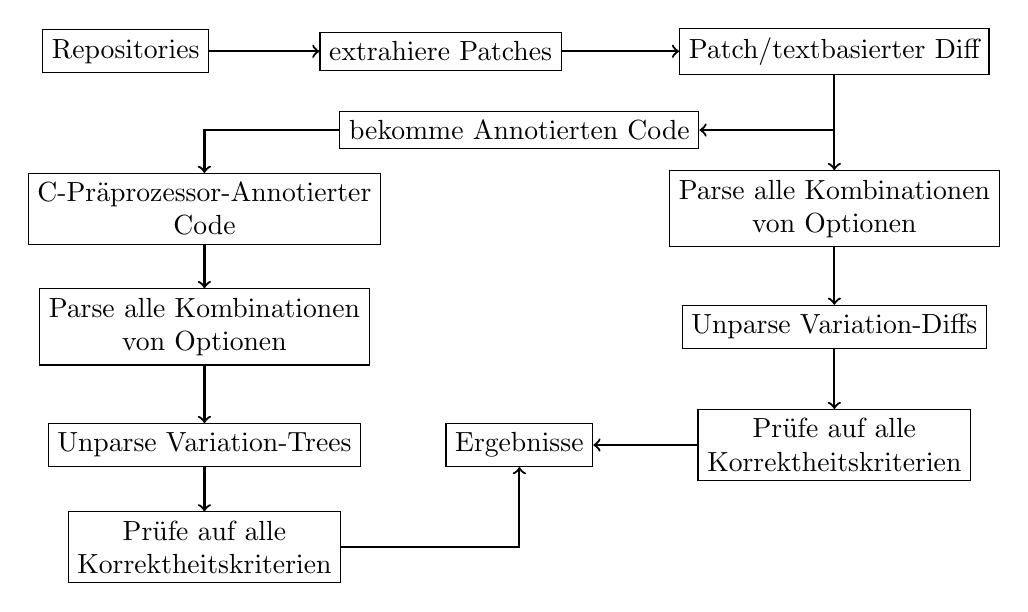
\begin{tikzpicture}
	\node[draw,align=center] (A) at (-1,0) {Repositories};
	\node[draw,align=center] (B) at (3,0) {extrahiere Patches};
	\node[draw,align=center] (C) at (8,0) {Patch/textbasierter Diff};
	\node[draw,align=center] (D) at (4,-1) {bekomme Annotierten Code};
	\node[draw,align=center] (E) at (0,-2) {C-Präprozessor-Annotierter\\ Code};
	\node[draw,align=center] (F) at (8,-2) {Parse alle Kombinationen \\von Optionen};
	\node[draw,align=center] (G) at (8,-3.5) {Unparse  Variation-Diffs};
	\node[draw,align=center] (H) at (8,-5) {Prüfe auf alle\\Korrektheitskriterien};
	\node[draw,align=center] (I) at (0,-3.5) {Parse alle Kombinationen \\von Optionen};
	\node[draw,align=center] (J) at (0,-5) {Unparse  Variation-Trees};
	\node[draw,align=center] (K) at (0,-6.3) {Prüfe auf alle\\Korrektheitskriterien};
	\node[draw,align=center] (L) at (4,-5) {Ergebnisse};
	
	\draw[thick,->] (A) -- (B);
	\draw[thick,->] (B) -- (C);
	\draw[thick,->] (C) |- (D);
	\draw[thick,->] (C) -- (F);
	\draw[thick,->] (D) -| (E);
	\draw[thick,->] (F) -- (G);
	\draw[thick,->] (G) -- (H);
	\draw[thick,->] (H) -- (L);
	\draw[thick,->] (E) -- (I);
	\draw[thick,->] (I) -- (J);
	\draw[thick,->] (J) -- (K);
	\draw[thick,->] (K) -| (L);
\end{tikzpicture}
\caption{Aufbau der Auswertung}
\end{figure}

\subsection{Ergebnisse}
In diesem Abschnitt wollen wir über die Ergebnisse der Auswertung berichten. Während der Auswertung wurden die Exceptions ausgelöst. Diese Exection wurden dadurch ausgelöst, dass was dem Parser übergeben wurde, nicht geparst werden konnte. Wenn irgendwas nicht geparst werden kann, dann ist es auch nicht für unsere Auswertung relevant und wird von uns ignoriert. Wir können nicht garantieren, dass die Exception nur dadurch ausgelöst wurden, aber keiner der Exceptions hat die Auswertung abgebrochen. Nachdem wir die Exceptions erwähnt haben, können wir zu den Ergebnissen der Auswertung kommen.\\

In der Tabelle 5.2 sind die Ergebnisse der Auswertung für C-Präprozessor-Annotierten Code zu sehen. Die Tabelle zeigt ganz oben die Anzahl der untersuchten C-Präprozessor-Annotierten Codes, das sind 98802. Danach auf der linken Seite der Tabelle sind die Optionen für den Parser zu sehen und ob diese ausgewählt wurden oder nicht. Auf der rechten Seite der Tabelle ist zu sehen, wie viel mal ein bestimmtes Korrektheitskriterium für die Kombination von Optionen erfühlt wurden. Die Spalte mit dem Fehler zeigt an wie viel mal für eine Kombination von Parser-Optionen keiner der von uns definierten Korrektheitskriterien erfühlt wurde.\\

\begin{table}[H]
	\resizebox{1\textwidth}{!}{
	\begin{tabular}{|ccccc|}
		\hline
		\multicolumn{4}{|c|}{Anzahl Ungeparster C-Präprozessor-Annotierter Codes}                                                                         & 98802 \\ \hline
		\multicolumn{2}{|c||}{Parser Optionen}                         & \multicolumn{3}{c|}{Ergebnisse der Auswertung für}                            \\ \hline
		\multicolumn{1}{|c|}{\parbox[][1.2cm][]{4cm}{ Collapse-Multiple-Code-Lines}} & \multicolumn{1}{c||}{Ignore-Empty-Lines} & \multicolumn{1}{c|}{Syntaktische Gleichheit} & \multicolumn{1}{c|}{\parbox[][1.2cm][]{4cm}{Syntaktische Gleichheit ohne Whitespace}} & Fehler \\ \hline
		\multicolumn{1}{|c|}{False} & \multicolumn{1}{c||}{False} & \multicolumn{1}{c|}{0} & \multicolumn{1}{c|}{98802} & 0 \\ \hline
		\multicolumn{1}{|c|}{True} & \multicolumn{1}{c||}{False} & \multicolumn{1}{c|}{0} & \multicolumn{1}{c|}{98802} & 0 \\ \hline
		\multicolumn{1}{|c|}{False} & \multicolumn{1}{c||}{True} & \multicolumn{1}{c|}{0} & \multicolumn{1}{c|}{98624} & 178 \\ \hline
		\multicolumn{1}{|c|}{True} & \multicolumn{1}{c||}{True} & \multicolumn{1}{c|}{0} & \multicolumn{1}{c|}{98624} & 178 \\ \hline
	\end{tabular}
}
\caption{Ergebnisse der Auswertung für das Unparsen von C-Präprozessor-Annotierten Code}
\end{table}


Die Ergebnisse der Auswertung für textbasierte Diffs sind in der Tabelle 5.2 zu sehen. Die Tabelle ist analog zu der Tabelle 5.2 aufgebaut. Oben in der Tabelle ist die Anzahl der untersuchten, textbasierten Diffs zu sehen. Die Anzahl beträgt 49401, welches die Hälfte der untersuchten C-Präprozessor-Annotierten Codes aus der Tabelle 5.2, da jeder textbasierter Diff aus zwei C-Präprozessor-Annotierten Codes besteht. Wie in der Tabelle 5.2 ist in der Tabelle 5.3 auch die Parser-Optionen und die ausgewählten Kombinationen gegeben. Rechts in der Tabelle sind die Korrektheitskriterien mit dem Fehler-Fall zu sehen. In der Tabelle 5.3 ist ein zu untersuchender Korrektheitskriterium mehr gegeben als in der Tabelle 5.2. \\
\begin{table}[h]
	\resizebox{1\textwidth}{!}{
	\begin{tabular}{|cccccc|}
		\hline
		\multicolumn{5}{|c|}{Anzahl Ungeparster textbasierter Diffs}                                                                                                 & 49401 \\ \hline
		\multicolumn{2}{|c||}{Parser Optionen}                         & \multicolumn{4}{c|}{Ergebnisse der Auswertung für}                                                    \\ \hline
		\multicolumn{1}{|c|}{\parbox[][1.2cm][]{3.2cm}{ Collapse-Multiple-Code-Lines}} & \multicolumn{1}{c||}{\parbox[][1.2cm][]{2.7cm}{Ignore-Empty-Lines}} & \multicolumn{1}{c|}{\parbox[][1.2cm][]{2.2cm}{Syntaktische Gleichheit}} & \multicolumn{1}{c|}{\parbox[][1.2cm][]{4cm}{Syntaktische Gleichheit ohne Whitespace}} & \multicolumn{1}{c|}{\parbox[][1.2cm][]{2.2cm}{Semantische Gleichheit}} & Fehler \\ \hline
		\multicolumn{1}{|c|}{False} & \multicolumn{1}{c||}{False} & \multicolumn{1}{c|}{0} & \multicolumn{1}{c|}{46514} & \multicolumn{1}{c|}{49390} & 11 \\ \hline
		\multicolumn{1}{|c|}{True} & \multicolumn{1}{c||}{False} & \multicolumn{1}{c|}{0} & \multicolumn{1}{c|}{46514} & \multicolumn{1}{c|}{49390} & 11 \\ \hline
		\multicolumn{1}{|c|}{False} & \multicolumn{1}{c||}{True} & \multicolumn{1}{c|}{0} & \multicolumn{1}{c|}{36778} & \multicolumn{1}{c|}{49300} & 101 \\ \hline
		\multicolumn{1}{|c|}{True} & \multicolumn{1}{c||}{True} & \multicolumn{1}{c|}{0} & \multicolumn{1}{c|}{36778} & \multicolumn{1}{c|}{49300} & 101 \\ \hline
	\end{tabular}
}
\caption{Ergebnisse der Auswertung für das Unparsen von textbasierten Diffs}
\end{table}

Es wurden 11 textbasierter Diffs sich gemerkt, welche als nicht unparsbar vermerkt wurden. So ein Fall tritt auf, wenn für einen textbasierten Diff keiner der Korrektheitskriterien für keine Kombination der Parse-Optionen erfühlt wurde. Wir haben alle diese nicht unparsbarer textbasierten Diffs näher betrachtet. Es hat sich herausgestellt das in all diesen Fällen es Probleme mit endif gab. Dabei war keiner dieser Fehlerfälle dadurch ausgelöst, da es zu einem if keinen endif gab.


\subsection{Diskussion}
Nachdem wir die Ergebnisse der Auswertung vorgestellt haben, sind wir in der Labe die Forschungsfrage zu beantworten. Unsere Forschungsfrage ist, wie Korrekt ist unser Unparser. \\

Damit wir diese Frage für das Unparsen von C-Präprozessor-Annotierten Code beantworten können, müssen wir die Tabelle 5.2 betrachten. Dabei ist für die Beantwortung der Frage nur Zeilen mit Kombinationen von Parser-Optionen Collapse-Multiple-Code-Lines ist False und Ignore-Empty-Lines ist False und Collapse-Multiple-Code-Lines ist True und Ignore-Empty-Lines ist False. Es sind nur diese beiden Zeilen von Bedeutung, da unsere Unparser darauf ausgerichtet ist, nur mit der Parser-Option Collapse-Multiple-Code-Lines Korrekt zu funktionieren, da in diesem Fall keine zusätzlichen Informationen verloren gehen, sondern nur etwas anders dargestellt werden, was unseren Unparser nicht stört. Bei der Parser-Option Ignore-Empty-Lines gibt es einen zusätzlichen Information-Verlust und um den wieder zu beheben, müssen wir diese Information speichern, welches den Sinn dieser Parser-Option widerspricht. Aus diesem Grund war die korrekte Arbeit unseren Unparser bei Auswahl dieser Option nicht vorgesehen, aber wir wollten trotzdem sehen, wie Korrekt er auch bei der Auswahl nicht vorgesehener Option funktioniert. Wenn wir jetzt die ersten beiden Parser-Kombinationen in der Tabelle 5.2 betrachte, sehen wir das die Werte der beiden Zeilen für das jeweilige Korrektheitskriterium gleich ist. Dabei sehen wir das die syntaktische Gleichheit kein einziges Mal erfühlt wurde, aber es auch keinen einzigen Fall gibt, dass der Unparser nicht funktioniert hat. Jedes Mal in der Auswertung konnte unser Unparser die syntaktische Gleichheit ohne Whitespace garantieren. Dies lässt uns zu dem Entschluss kommen, dass unser Unparser für das Unparsen von C-Präprozessor-Annotierten Code korrekt funktioniert. Diese Entscheidung basiert auf dem, das bei dem Entfernen von Whitespace nicht alle Whitespace-Zeichen entfernt werde, sondern nur bestimmt und das nach dieser Manipulation wir trotzdem einen C-Präprozessor-Annotierten Code erhalten. Wir vermuten, dass der Grund warum kein einziges Mal die syntaktische Korrektheit erfühlt, daran liegt das der Parser, auch wenn die Option Ignore-Empty-Lines nicht ausgewählt wurde, die letzten Zeilen, wenn sie leer sind, nicht speichert und deshalb kann unser Unparser das nicht syntaktisch korrekt wider herstellen, da ihn diese Informationen fehlen. Aus der Tabelle 5.2 können wir auch entnehmen wie Korrekt unser Unparser  bei der ausgewählten Parser-Option Ignore-Empty-Lines arbeitet. Dabei sehen wir das auch hier kein einziges Mal die syntaktische Gleichheit erreicht wurde, aber nicht wie in dem anderen Fällen, gibt es, hier Fälle welcher unser Unparser nicht korrekt unparsen konnte. Das sind 178 Fälle, welches 0,2$\%$ aller untersuchten Fälle darstellt. Für uns ist das der Grund genug zu sagen, das auch bei dieser Option unser unparser gut funktioniert. Bei der Kombination der Parser-Optionen wo beide Optionen ausgewählt sind, ist zu erkennen das die Werte, zu der vorherigen Kombination gleich sind. Es sind wieder 178 Fälle gegeben, welche nicht ungepoarst werden können, das müssen dieselben Fälle wie in vorherigen Fall sein, da bei ersten baiden Kombinationen es keine nicht unparsbaren Fälle gibt. Damit lässt sich sagen, dass unser Unparser korrekt für die vorgesehenen Kombinationen von Parser-Optionen funktioniert, aber das der auch gut für nicht vorgesehenen Kombinationen von Parser-Optionen arbeitet.\\

Nachdem wir die Forschungsfrage für das Unparsen von C-Präprozessor-Annotierten Code beantwortet haben, müssen wir das noch für das Parsen von textbasierten Diffs beantworten. Dazu gehen wir analog zu dem vorherigen Mal von und schauen und die Tabelle 5.3 an. In dieser Tabelle sind für die Beantwortung der Frage nur die ersten beiden Kombinationen von Parser-Optionen relevant. Aus dem Grund das wie in vorherigen Mal unser Unparser nur für die mit diesen Kombinationen entwickelt wurde. Es ist zu sehen das kein einziges Mal die syntaktische Gleichheit erfühlt wurde, der Grund dafür könnte derselbe wie für das Unparsen von C-Präprozessor-Annotierten Code sein. Dabei haben wir aber Fälle, welche nicht ungeparst werden konnten. Wir haben und diese Fälle angeschaut und herausgefunden, das die Probleme bei endif auftauchen. Dabei geschieht dies Problem innerhalb eines textbasierten Diff anhand dieser Fehlerfälle nur maximal 2 Mal. Diese Probleme beziehen sich dabei aber nicht darauf das ein if kein dazugehöriges endif nicht hat. Die betrachteten Probleme enthielten, falsche Einrückung, falsche Positionierung, falsche oder fehlen der Kommentare und abweichende Darstellung von endif. Es lässt sich Vermuten das Teil dieser Probleme damit zusammen hängen, das wir die textbasierte Diff nicht selbst Unparsen, sondern diese Aufgabe auf das Unparsen von C-Präprozessor-Annotierten Code reduzieren und mit diesen einen textbasierten Diff bilden. Abhängig davon welcher Algorithmus dazu verwendet wurde, können unterschiedliche textbasierte Diffs herauskommen. Ein weiterer Grund für einige der Probleme könnte sein, dass wir bei der Erweiterung der Parser Implementierung nicht alles beachtet haben und in bestimmten Fällen, welche wir anhand der Fehlerfälle nicht erkennen konnten, die Information von endif nicht korrekt gespeichert wird. Aus den Grunden das die Fehlerfälle weniger als 0,03$\%$ alle untersuchten textbasierten Diffs darstellen, das alle Probleme nur bei den endif stattfinden und das dabei immer ein endif zu seinem if vorhanden ist, können wir sagen das diese Fehler für die Entscheidung, ob unser unparser korrekt ist zu vernachlässigen sind. In den ersten beiden Kombinationen von Parser-Optionen sind noch syntaktische Gleichheit ohne Whitespace und semantische Gleichheit zu sehen, für beide Kombinationen sind die Werte gleich. Dabei sehen wir, dass die syntaktische Gleichheit ohne Whitespace nicht gleich der semantischen Gleichheit ist. Der Grund dafür könnte sein, dass Abhängig davon wie der Algorithmus für das Bilden von textbasierten Diffs in unseren Unparser funktioniert, es vorkommen kann das, wenn der Inhalt eine Zeile durch einen anderen ersetzt wurde, dann könne diese Information das es entfernt und wieder hinzugefügt worden sein, unterschiedlich dargestellt werden, was eine semantisch Gleichen textbasierten Diff liefert aber nicht der syntaktischen Gleichheit ohne Whitespace entspricht. Für die Kombination von Parser-Optionen wo Ignore-Empty-Lines verwendet wird, lässt sich sehen, das unser Unparser sich auch hier es schafft, größtenteils korrekt unzuparsen und das nur ungefähr 0,2$\%$ aller betrachteten textbasierten Diffs nicht geschaft wurden, korrekt unzuparsen. Aus der gegebenen Information lässt sich von uns aus ein Schluss ziehe, dass unser Unparser trotz den Fehler sich gut für das Unpaser von textbasierten Diffs eignet. 
%interpretation der Ergebnisse
%Beantworten der Forschungsfrage

\section{Zusammenfassung}

In diesem Kapitel haben wir unsere Definition von Korrektheitskriterien für den Unparser vorgestellt. Wie diese Korrektheitskriterien angewandt werden müssen und wie diese zusammenhängen. Die Korrektheitskriterien sind syntaktische Gleichheit, syntaktische Gleichheit und semantische Gleichheit. Dazu haben wir eine Auswertung beschrieben und durchgeführt, um anhand der Korrektheitsriterien zu prüfen, ob unser Unparser korrekt funktioniert.








